% SPDX-License-Identifier: CC-BY-4.0
%
% Copyright (c) 2023 Nelson Vieira
%
% @author Nelson Vieira <2080511@student.uma.pt>
% @license CC-BY-4.0 <https://creativecommons.org/licenses/by/4.0/legalcode.txt>
\section{Discussion}\label{section:discussion}

\par
This chapter serves to discusses the main takeaways found in the literature
review and address the results of the questionnaire and the usability tests,
and any other interesting remarks found during the course of this work. The
research questions that were posed in Chapter \ref{introduction} will also
be addressed.

\subsection{SLR Findings}

There has been a rising interest by research papers in addressing privacy
issues or challenges in the Internet of Things, at least since 2015-2016
where the number or papers jumped from 11 600 in 2015 to 19 400 in 2016
and rising since then until reaching a peak of 74 400 in 2020 and slightly
declining since then, and at least until August of 2023 there have been
around 36 000 papers published, according to the data seen in Figure \ref{fig:iotprivacy_papers}.

\begin{figure}
    \begin{center}
        \pgfkeys{/pgf/number format/1000 sep={\,}}
        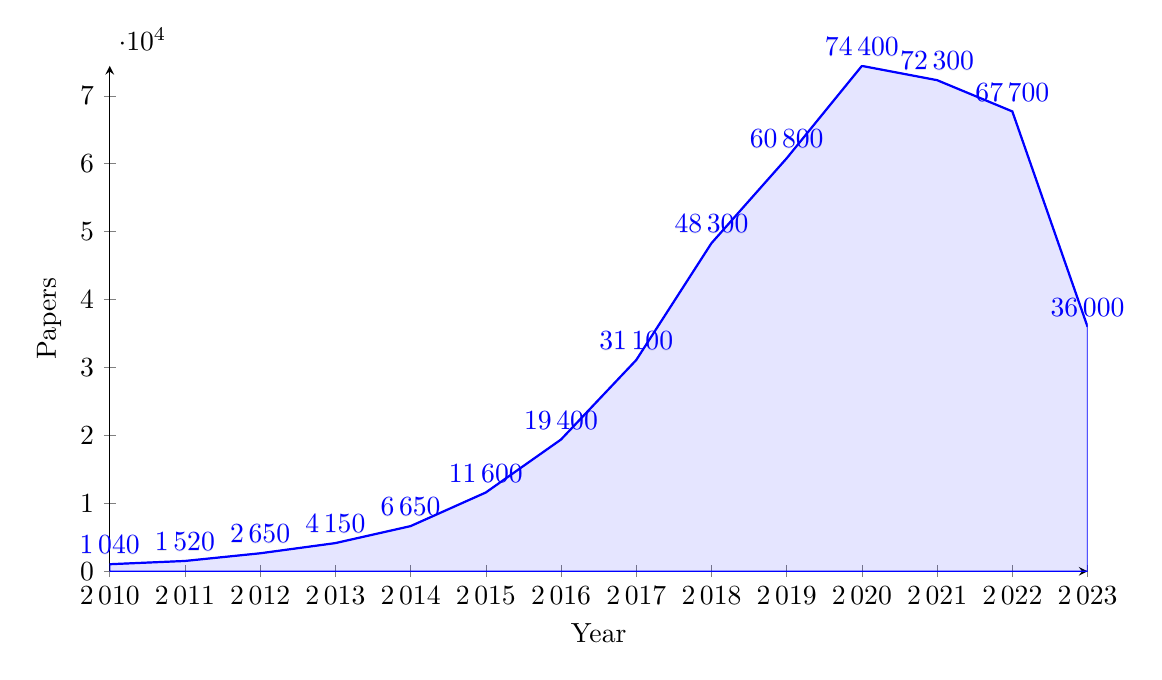
\begin{tikzpicture}
            \begin{axis}[
                width=14cm,
                height=8cm,
                xmin=2010,
                xmax=2023,
                ymin=0,
                ymax=74400,
                xlabel=Year,
                ylabel=Papers,
                axis x line=bottom,
                axis y line=left,
                nodes near coords={\pgfmathprintnumber[fixed]\pgfplotspointmeta}
            ]
            \addplot[draw=blue,samples=100,fill=blue,fill opacity=0.1] coordinates {(2010,1040) (2011,1520) (2012,2650) (2013,4150) (2014,6650) (2015,11600) (2016,19400) (2017,31100) (2018,48300) (2019,60800) (2020,74400) (2021,72300) (2022,67700) (2023,36000)}\closedcycle;
            \addplot[blue,thick,samples=100,domain=2010:2023] coordinates {(2010,1040) (2011,1520) (2012,2650) (2013,4150) (2014,6650) (2015,11600) (2016,19400) (2017,31100) (2018,48300) (2019,60800) (2020,74400) (2021,72300) (2022,67700) (2023,36000)};
            \end{axis}
        \end{tikzpicture}
        \caption{Distribution of papers, per year since 2010, on privacy in the Internet of Things, based on Google Scholar database results.}
        \label{fig:iotprivacy_papers}
    \end{center}
\end{figure}

Figure \ref{fig:privacy_keywords_papers} depicts the number of publications
per topic in multiple databases, all of which are still related to the main
theme of privacy in the IoT, particularly Google Scholar, BASE, and CORE. This
data is from papers since 2020, the database with the most papers is Google Scholar
followed by the distant second BASE and finally
CORE with the smallest number of papers. Around 249000 papers exist discussing privacy
in the IoT in Google Scholar, 20641 papers on CORE and 8014 on BASE, from these papers
the most researched topic has been security with around 196000 papers on Google Scholar,
17738 on CORE and 5600 on BASE. This data cannot be accepted at face value because
searches on these databases are conducted using keywords, these keywords may occur
in the title of the work or on the content, but this does not imply that the work
is about keywords in general, rather, it simply indicates that the keywords appear
on the work. But it can represent a rough estimate of what is being researched.
Other databases were used in course of the research like Semantic Scholar,
Baidu Scholar and RefSeek but these databases do not have good
filters for advanced searching and/or have a small number of papers.

There is a big focus on security, AI and blockchain in recent literature,
specially from 2020 onward. Some studies \cite{dadkhah2020publications, duygu2023analysis} have
focused on this type of analysis.

\begin{figure}[H]
    \begin{center}
        \pgfkeys{/pgf/number format/1000 sep={\,}}
        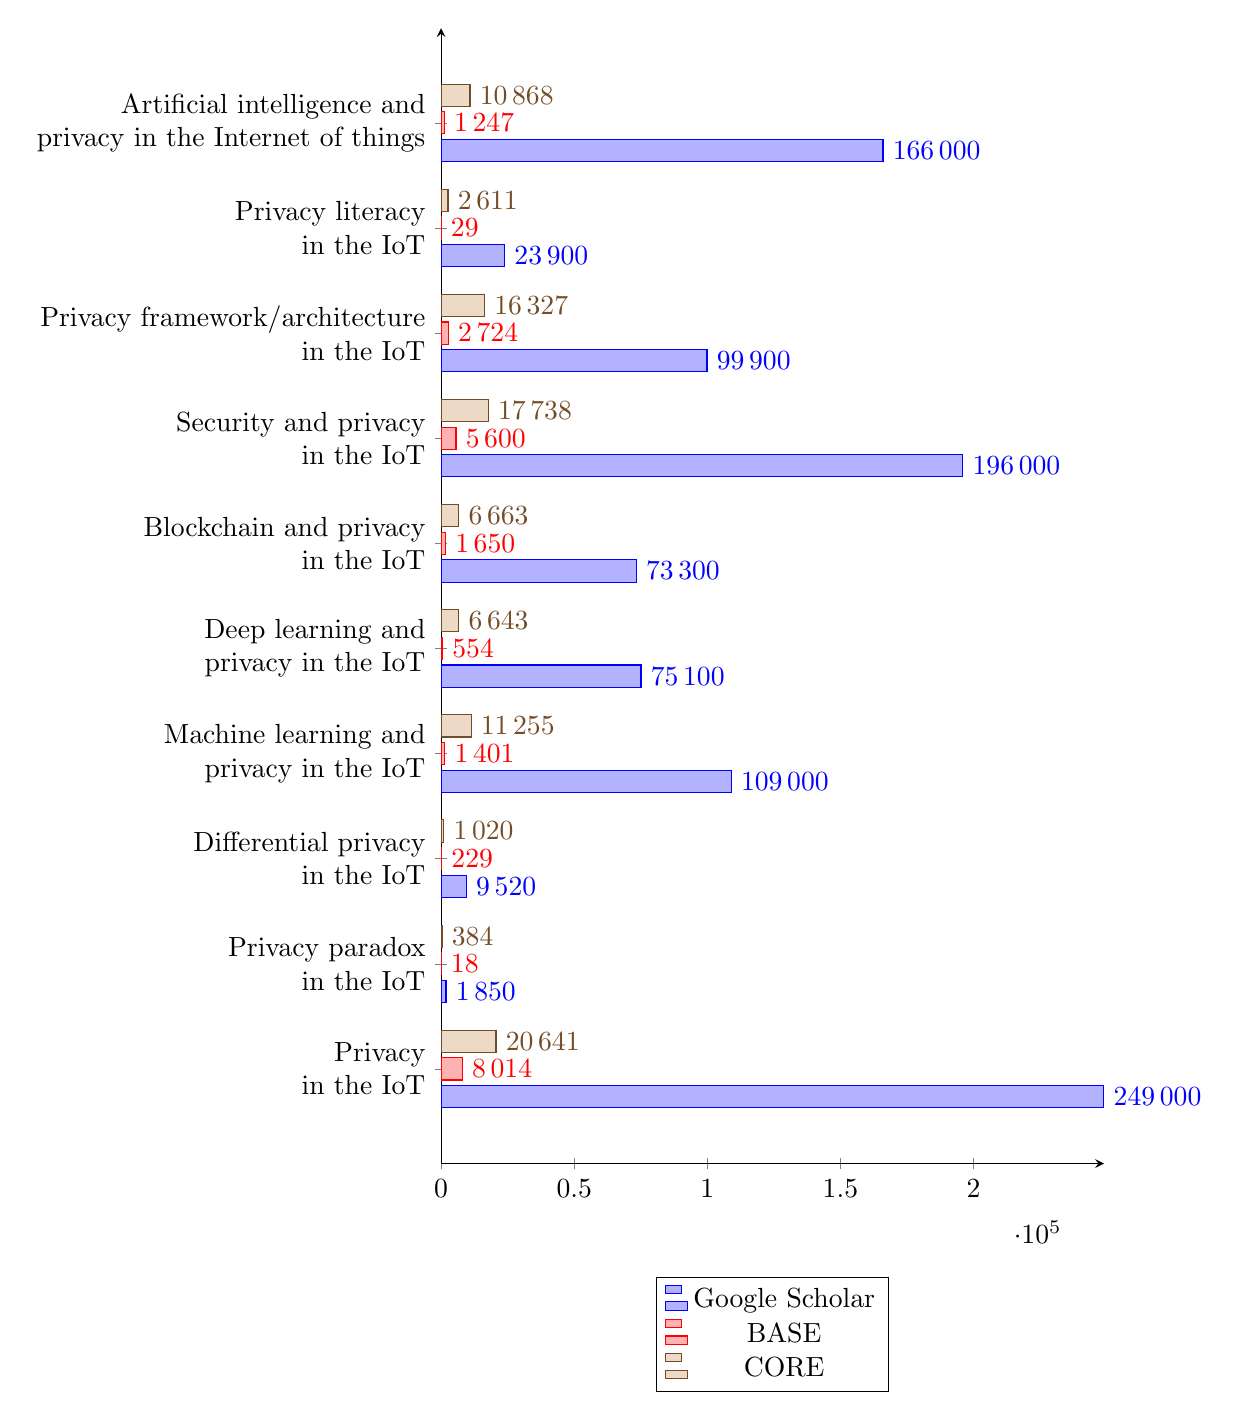
\begin{tikzpicture}
            \begin{axis}[
                width=10cm,
                height=16cm,
                xbar,
                xmin=0,
                symbolic y coords={Privacy in the IoT,Privacy paradox in the IoT,Differential privacy in the IoT,Machine learning and privacy in the IoT,Deep learning and privacy in the IoT,Blockchain and privacy in the IoT,Security and privacy in the IoT,Privacy framework/architecture in the IoT,Privacy literacy in the IoT,Artificial intelligence and privacy in the Internet of things},
                ytick=data,
                yticklabels={
                    Privacy\\in the IoT,
                    Privacy paradox\\in the IoT,
                    Differential privacy\\in the IoT,
                    Machine learning and\\privacy in the IoT,
                    Deep learning and\\privacy in the IoT,
                    Blockchain and privacy\\in the IoT,
                    Security and privacy\\in the IoT,
                    Privacy framework/architecture\\in the IoT,
                    Privacy literacy\\in the IoT,
                    Artificial intelligence and\\privacy in the Internet of things,
                },
                yticklabel style={align=right},
                bar width=8pt,
                axis x line=bottom,
                axis y line=left,
                xticklabel style={/pgf/number format/fixed},
                enlarge y limits=0.1,
                nodes near coords={\pgfmathprintnumber[fixed]\pgfplotspointmeta},
                legend style={at={(0.5,-0.1)},anchor=north},
                % ticklabel style={font=\tiny},
            ]
                \addplot coordinates {(249000,Privacy in the IoT) (1850,Privacy paradox in the IoT) (9520,Differential privacy in the IoT) (109000,Machine learning and privacy in the IoT) (75100,Deep learning and privacy in the IoT) (73300,Blockchain and privacy in the IoT) (196000,Security and privacy in the IoT) (99900,Privacy framework/architecture in the IoT) (23900,Privacy literacy in the IoT) (166000,Artificial intelligence and privacy in the Internet of things)};
                \addlegendentry{Google Scholar}
                \addplot coordinates {(8014,Privacy in the IoT) (18,Privacy paradox in the IoT) (229,Differential privacy in the IoT) (1401,Machine learning and privacy in the IoT) (554,Deep learning and privacy in the IoT) (1650,Blockchain and privacy in the IoT) (5600,Security and privacy in the IoT) (2724,Privacy framework/architecture in the IoT) (29,Privacy literacy in the IoT) (1247,Artificial intelligence and privacy in the Internet of things)};
                \addlegendentry{BASE}
                \addplot coordinates {(20641,Privacy in the IoT) (384,Privacy paradox in the IoT) (1020,Differential privacy in the IoT) (11255,Machine learning and privacy in the IoT) (6643,Deep learning and privacy in the IoT) (6663,Blockchain and privacy in the IoT) (17738,Security and privacy in the IoT) (16327,Privacy framework/architecture in the IoT) (2611,Privacy literacy in the IoT) (10868,Artificial intelligence and privacy in the Internet of things)};
                \addlegendentry{CORE}
            \end{axis}
        \end{tikzpicture}
        \caption{Distribution of papers on privacy in IoT, since 2020, by keyword searches on Google Scholar, BASE and CORE databases.}
        \label{fig:privacy_keywords_papers}
    \end{center}
\end{figure}

Chapter \ref{section:state_of_the_art} discussed many works that addressed privacy challenges in the
IoT and some that proposed approaches to address these issues. The current chapter assesses
different aspects of the included papers including their general information,
purpose, intended application, issues that still exist, and any other comments
that should be taken into account.

Table \ref{table:literature_overview} displays general information about the
papers that were included \cite{wilson2012unpacking, warshaw2015can, lee2015privacy, acquisti2007can, knijnenburg2013dimensionality, wakefield2013influence, flender2012type, dienlin2015privacy, baek2014solving, taddicken2014privacy, norberg2007privacy, kokolakis2017privacy, brandimarte2013misplaced, xie2019consumers, SCHWAIG20131, sannon2018privacy, ZhaoSurvey, zhao2020local, Gupta2022Privacy, Kuhtreiber2022survey, sicari2015security, LinSurvey, yang2022overview, zubaydi2023leveraging, khanna2020internet, tzafestas2018ethics, ziegeldorf2014privacy, naeini2017privacy, koohang2022internet, SkirpanPrivacy, WEBER2015618, FabianoInternet, weber2010internet, hadzovic2023path, SunSecure, xiong2018defending, AntunesFederated, opara2022framework, perera2020designing, zhang2017privacy, zhang2019security, yu2018blockchain, AliIoT, ColnagoInforming, FengDesign, DasPersonalized, ZhuIntegrating, electronics12122589, KumarLTE}.
It is discernible that 22\% of the total papers were published in 2022 \cite{ZhaoSurvey, Gupta2022Privacy, Kuhtreiber2022survey, yang2022overview, zubaydi2023leveraging, koohang2022internet, SkirpanPrivacy, SunSecure, AntunesFederated, opara2022framework, ZhuIntegrating},
while 12\% of the papers were published in 2017 \cite{kokolakis2017privacy, LinSurvey, naeini2017privacy, FabianoInternet, zhang2017privacy, AliIoT},
with 12\% as well as in 2018 \cite{sannon2018privacy, tzafestas2018ethics, xiong2018defending, yu2018blockchain, DasPersonalized, Qu2018Privacy}
and in 2015 \cite{warshaw2015can, lee2015privacy, dienlin2015privacy, sicari2015security, WEBER2015618, perera2015big},
there were 8\% of papers published in 2013 \cite{knijnenburg2013dimensionality, wakefield2013influence, brandimarte2013misplaced, SCHWAIG20131},
with the same percentage in 2014 \cite{baek2014solving, taddicken2014privacy, ziegeldorf2014privacy, KumarLTE}
and in 2020 \cite{zhao2020local, khanna2020internet, perera2020designing, ColnagoInforming},
the remaining 18\% of papers were published between the years 2010 \cite{weber2010internet},
2012 \cite{wilson2012unpacking, flender2012type}, 2019 \cite{xie2019consumers, zhang2019security},
2021 \cite{FengDesign} and 2023 \cite{hadzovic2023path, electronics12122589},
with the exception of a small percentage of 2.08\% being published in 2007 \cite{norberg2007privacy}.
Overall, 38\% of the literature originate from the United States of America (USA) \cite{wilson2012unpacking, warshaw2015can, knijnenburg2013dimensionality, wakefield2013influence, norberg2007privacy, brandimarte2013misplaced, xie2019consumers, SCHWAIG20131, sannon2018privacy, Gupta2022Privacy, naeini2017privacy, koohang2022internet, SkirpanPrivacy, xiong2018defending, opara2022framework, ColnagoInforming, FengDesign, DasPersonalized, KumarLTE},
10\% originate from China \cite{LinSurvey, SunSecure, zhang2017privacy, zhang2019security, yu2018blockchain},
10\% are from Germany \cite{flender2012type, dienlin2015privacy, taddicken2014privacy, Kuhtreiber2022survey, ziegeldorf2014privacy}
and 42\% are spread across 13 different countries \cite{lee2015privacy, baek2014solving, kokolakis2017privacy, ZhaoSurvey, zhao2020local, sicari2015security, yang2022overview, zubaydi2023leveraging, khanna2020internet, tzafestas2018ethics, WEBER2015618, FabianoInternet, weber2010internet, hadzovic2023path, AntunesFederated, perera2020designing, AliIoT, ZhuIntegrating, electronics12122589}.
The majority of the included papers, 74\% \cite{lee2015privacy, knijnenburg2013dimensionality, wakefield2013influence, dienlin2015privacy, baek2014solving, taddicken2014privacy, norberg2007privacy, kokolakis2017privacy, brandimarte2013misplaced, xie2019consumers, SCHWAIG20131, ZhaoSurvey, zhao2020local, Gupta2022Privacy, Kuhtreiber2022survey, sicari2015security, LinSurvey, yang2022overview, zubaydi2023leveraging, khanna2020internet, tzafestas2018ethics, ziegeldorf2014privacy, koohang2022internet, WEBER2015618, weber2010internet, hadzovic2023path, SunSecure, AntunesFederated, perera2020designing, zhang2017privacy, zhang2019security, yu2018blockchain, DasPersonalized, ZhuIntegrating, electronics12122589},
are published in journals, while 24\% are published in conferences \cite{wilson2012unpacking, warshaw2015can, flender2012type, sannon2018privacy, naeini2017privacy, FabianoInternet, xiong2018defending, opara2022framework, AliIoT, ColnagoInforming, FengDesign, KumarLTE},
and 2\% in a magazine \cite{SkirpanPrivacy}.
The publishers' information is provided so that the database of origin
can be easily accessed. The ACM database \cite{warshaw2015can, sannon2018privacy, ZhaoSurvey, SkirpanPrivacy, SunSecure, AntunesFederated, opara2022framework, zhang2019security, AliIoT, ColnagoInforming, FengDesign, ZhuIntegrating, KumarLTE}
provides 26\% of all publications, followed by Elsevier \cite{lee2015privacy, knijnenburg2013dimensionality, wakefield2013influence, baek2014solving, kokolakis2017privacy, SCHWAIG20131, Kuhtreiber2022survey, sicari2015security, koohang2022internet, WEBER2015618, weber2010internet, perera2020designing}
with 24\%, IEEE \cite{zhao2020local, Gupta2022Privacy, LinSurvey, FabianoInternet, hadzovic2023path, xiong2018defending, zhang2017privacy, yu2018blockchain, DasPersonalized}
with 22\%, MDPI \cite{zubaydi2023leveraging, tzafestas2018ethics, electronics12122589}
with 6\% and Wiley \cite{dienlin2015privacy, norberg2007privacy, ziegeldorf2014privacy}
with the same percentage, and 16\% are divided between the other 7 publishers \cite{wilson2012unpacking, flender2012type, taddicken2014privacy, brandimarte2013misplaced, xie2019consumers, yang2022overview, khanna2020internet, naeini2017privacy}.\\

% * 50 papers in total
\begin{footnotesize}
    \begin{longtable}{p{1.2cm} p{1cm} p{1.6cm} p{3.2cm} p{5cm} p{3cm}}
        \hline
        \textbf{Ref $\#$} & \textbf{Year} & \textbf{Country} & \textbf{Publication Type} & \textbf{Publisher} & \textbf{Scope} \\
        \hline
        \endfirsthead
        \multicolumn{6}{@{}l}{\dots continued}\\\hline
        \textbf{Ref $\#$} & \textbf{Year} & \textbf{Country} & \textbf{Publication Type} & \textbf{Publisher} & \textbf{Scope} \\
        \hline
        \endhead
        \multicolumn{6}{r@{}}{continues \ldots}\\
        \endfoot
        \endlastfoot
        % \cite{DarrenState} & 2015 & USA & Report & \textbf{Norton} NortonLifeLock & Statistical analisys \\
        % \hline
        % \cite{solove2021myth} & 2021 & USA & Journal & \textbf{George Washington University} George Washington Law Review & Privacy paradox \\
        % \hline
        % \cite{WilliamsPrivacy} & 2017 & UK & Conference & \textbf{IEEE} 15th Annual Conference on Privacy, Security and Trust (PST) & Privacy paradox \\
        % \hline
        % \cite{lee2021investigating} & 2021 & South Korea & Journal & \textbf{MDPI} Sustainability & Privacy paradox \\
        % \hline
        % \cite{goad2021privacy} & 2021 & Australia & Journal & \textbf{Elsevier} Information \& Management & Privacy paradox \\
        % \hline
        % \cite{gerber2018explaining} & 2018 & USA & Journal & \textbf{Elsevier} Computers \& security & Privacy paradox \\
        % \hline
        \cite{wilson2012unpacking} & 2012 & USA & Conference & \textbf{AIS} 33rd International Conference on Information Systems & Privacy paradox \\
        \hline
        \cite{warshaw2015can} & 2015 & USA & Conference & \textbf{ACM} Proceedings of the 33rd Annual ACM Conference on Human Factors in Computing Systems & Privacy paradox \\
        \hline
        \cite{lee2015privacy} & 2015 & South Korea & Journal & \textbf{Elsevier} Expert Systems with Applications & Privacy paradox and healthcare \\
        \hline
        % \cite{zak2008moral} & 2008 & USA & Book & \textbf{Princeton University Press} & Morality in economy \\
        % \hline
        % \cite{acquisti2007can} & 2007 & USA & Book & \textbf{Auerbach Publications} & Digital Privacy \\
        % \hline
        \cite{knijnenburg2013dimensionality} & 2013 & USA & Journal & \textbf{Elsevier} International Journal of Human-Computer Studies & Privacy paradox \\
        \hline
        \cite{wakefield2013influence} & 2013 & USA & Journal & \textbf{Elsevier} The Journal of Strategic Information Systems & Privacy paradox \\
        \hline
        \cite{flender2012type} & 2012 & Germany & Conference & \textbf{Springer} International Symposium on Quantum Interaction & Privacy paradox \\
        \hline
        \cite{dienlin2015privacy} & 2015 & Germany & Journal & \textbf{Wiley} European Journal of Social Psychology & Privacy paradox \\
        \hline
        \cite{baek2014solving} & 2014 & South Korea & Journal & \textbf{Elsevier} Computers in Human Behavior & Privacy paradox \\
        \hline
        \cite{taddicken2014privacy} & 2014 & Germany & Journal & \textbf{Oxford University Press} Journal of Computer-Mediated Communication & Privacy paradox \\
        \hline
        \cite{norberg2007privacy} & 2007 & USA & Journal & \textbf{Wiley} Journal of Consumer Affairs & Privacy paradox \\
        \hline
        \cite{kokolakis2017privacy} & 2017 & Greece & Journal & \textbf{Elsevier} Computers \& security & Privacy paradox \\
        \hline
        \cite{brandimarte2013misplaced} & 2013 & USA & Journal & \textbf{SAGE Publications} Social Psychological and Personality Science & Privacy paradox \\
        \hline
        \cite{xie2019consumers} & 2019 & USA & Journal & \textbf{Taylor \& Francis} Journal of Interactive Advertising & Privacy paradox \\
        \hline
        \cite{SCHWAIG20131} & 2013 & USA & Journal & \textbf{Elsevier} Information \& Management & Online behaviour \\
        \hline
        % \cite{kearns2019ethical} & 2019 & UK & Book & \textbf{Oxford University Press} & Privacy algorithms \\
        % \hline
        \cite{sannon2018privacy} & 2018 & USA & Conference & \textbf{ACM} Proceedings of the 2018 CHI Conference on Human Factors in Computing Systems & Privacy paradox \\
        \hline
        \cite{ZhaoSurvey} & 2022 & Australia & Journal & \textbf{ACM} Computing Surveys & Differential Privacy \\
        \hline
        \cite{zhao2020local} & 2020 & Singapore & Journal & \textbf{IEEE} Internet of Things Journal & Differential Privacy, Federated Learning \\
        \hline
        % \cite{FromeLarge} & 2009 & USA & Conference & \textbf{IEEE} International Conference on Computer Vision & Image Protection \\
        % \hline
        % \cite{poddar2020visor} & 2020 & USA & Conference & \textbf{USENIX} Proceedings of the 29th USENIX Security Symposium & Video Analytics \\
        % \hline
        % \cite{ShokriPrivacy} & 2015 & USA & Conference & \textbf{ACM} Proceedings of the 22nd ACM SIGSAC Conference on Computer and Communications Security & Machine learning \\
        % \hline
        \cite{Gupta2022Privacy} & 2022 & USA & Journal & \textbf{IEEE} Internet of Things Journal & Systematic Literature Review \\
        \hline
        \cite{Kuhtreiber2022survey} & 2022 & Germany & Journal & \textbf{Elsevier} Pervasive and Mobile Computing & Systematic Literature Review \\
        \hline
        \cite{sicari2015security} & 2015 & Italy & Journal & \textbf{Elsevier} Computer Networks & Systematic Literature Review \\
        \hline
        \cite{LinSurvey} & 2017 & China & Journal & \textbf{IEEE} Internet of Things Journal & Systematic Literature Review \\
        \hline
        \cite{yang2022overview} & 2022 & Norway & Journal & \textbf{Frontiers} Frontiers in Artificial Intelligence & Systematic Literature Review \\
        \hline
        \cite{zubaydi2023leveraging} & 2022 & Hungary & Journal & \textbf{MDPI} Sensors & Systematic Literature Review \\
        \hline
        \cite{khanna2020internet} & 2020 & India & Journal & \textbf{Springer} Wireless Personal Communications & Systematic Literature Review \\
        \hline
        \cite{tzafestas2018ethics} & 2018 & Greece & Journal & \textbf{MDPI} Smart cities & Literature Review \\
        \hline
        % \cite{porras2018security} & 2018 & Finland & Conference & \textbf{AIS} Proceedings of the 51st Hawaii International Conference on System Sciences & Systematic Mapping Review \\
        % \hline
        % \cite{ahmed2019aspects} & 2019 & Czech Republic & Journal & \textbf{IEEE} Access & Systematic Mapping Review \\
        % \hline
        \cite{ziegeldorf2014privacy} & 2014 & Germany & Journal & \textbf{Wiley} Security and Communication Networks & Systematic Literature Review \\
        \hline
        \cite{naeini2017privacy} & 2017 & USA & Conference & \textbf{USENIX} Proceedings of the Thirteenth Symposium on Usable Privacy and Security & User awareness \\
        \hline
        \cite{koohang2022internet} & 2022 & USA & Journal & \textbf{Elsevier} International Journal of Information Management & User awareness \\
        \hline
        % \cite{tsourela2020internet} & 2020 & Greece & Journal & \textbf{MDPI} Future Internet & User awareness \\
        % \hline
        % \cite{knijnenburg2022modern} & 2022 & USA & Book & \textbf{Springer} & User awareness \\
        % \hline
        \cite{SkirpanPrivacy} & 2022 & USA & Magazine & \textbf{ACM} Communications of the ACM & User awareness \\
        \hline
        \cite{WEBER2015618} & 2015 & Switzerland & Journal & \textbf{Elsevier} Computer Law \& Security Review & Legislation \\
        \hline
        \cite{FabianoInternet} & 2017 & Italy & Conference & \textbf{IEEE} International Conference on Internet of Things (iThings) and IEEE Green Computing and Communications (GreenCom) and IEEE Cyber, Physical and Social Computing (CPSCom) and IEEE Smart Data (SmartData) & Legislation \\
        \hline
        \cite{weber2010internet} & 2010 & Switzerland & Journal & \textbf{Elsevier} Computer Law \& Security Review & Legislation \\
        \hline
        \cite{hadzovic2023path} & 2023 & Bosnia and Herzegovina & Journal & \textbf{IEEE} Communications Magazine & Legislation \\
        \hline
        % \cite{european2021europe} & 2021 & Belgium & Web & \textbf{European Commission} & Legislation \\
        % \hline
        \cite{SunSecure} & 2022 & China & Journal & \textbf{ACM} Transactions on Sensor Networks & Security \\
        \hline
        \cite{xiong2018defending} & 2018 & USA & Conference & \textbf{IEEE} 2018 IEEE International Conference on Acoustics, Speech and Signal & Security \\
        \hline
        \cite{AntunesFederated} & 2022 & Brazil & Journal & \textbf{ACM} Transactions on Intelligent Systems and Technology & Healthcare \\
        \hline
        % \cite{ChenSecurity} & 2021 & China & Journal & \textbf{IEEE} Internet of Things Journal & Healthcare \\
        % \hline
        \cite{opara2022framework} & 2022 & USA & Conference & \textbf{ACM} Proceedings of the 37th ACM/SIGAPP Symposium on Applied Computing & Framework \\
        \hline
        \cite{perera2020designing} & 2020 & UK & Journal & \textbf{Elsevier} Information Sciences & Framework \\
        \hline
        % \cite{o2017privacy} & 2017 & Ireland & Conference & \textbf{Elsevier} Procedia Computer Science & Framework \\
        % \hline
        % \cite{cavoukian2016embedding} & 2016 & Canada & Web & \textbf{Ryerson University} Privacy and Big Data Institute & Framework \\
        % \hline
        % \cite{alkhariji2023semantics} & 2023 & UK & Journal & \textbf{Elsevier} Future Generation Computer Systems & Framework \\
        % \hline
        % \cite{aljeraisy2021privacy} & 2021 & UK & Journal & \textbf{ACM} Computing Surveys & Framework \\
        % \hline
        \cite{zhang2017privacy} & 2017 & China & Journal & \textbf{IEEE} Internet of Things Journal & Framework \\
        \hline
        % \cite{barrett2018framework} & 2018 & USA & Tech Report & \textbf{NIST} Cybersecurity Framework & Framework \\
        % \hline
        % \cite{iso2022cybersecurity} & 2022 & Switzerland & Tech Report & \textbf{ISO} IT Security & IT Standards \\
        % \hline
        % \cite{iso2023privacysearch} & 2023 & Switzerland & Web & \textbf{ISO} & IT Standards \\
        % \hline
        % \cite{iso2023securitysearch} & 2023 & Switzerland & Web & \textbf{ISO} & IT Standards \\
        % \hline
        % \cite{sun2021survey} & 2021 & China & Journal & \textbf{IEEE} Network & Blockchain \\
        % \hline
        % \cite{mercer2016privacy} & 2016 & UK & Master's Report & \textbf{University College London} & Blockchain \\
        % \hline
        % \cite{stone2021trustless} & 2021 & USA & Web & \textbf{Cornell University} arXiv preprint arXiv:2102.04660 & Blockchain \\
        % \hline
        \cite{zhang2019security} & 2019 & China & Journal & \textbf{ACM} Computing Surveys & Blockchain \\
        \hline
        \cite{yu2018blockchain} & 2018 & China & Journal & \textbf{IEEE} Wireless Communications & Blockchain \\
        \hline
        \cite{AliIoT} & 2017 & Italy & Conference & \textbf{ACM} Proceedings of the Seventh International Conference on the Internet of Things & Blockchain \\
        \hline
        \cite{ColnagoInforming} & 2020 & USA & Conference & \textbf{ACM} Proceedings of the 2020 CHI Conference on Human Factors in Computing Systems & Privacy Assistant \\
        \hline
        \cite{FengDesign} & 2021 & USA & Conference & \textbf{ACM} Proceedings of the 2021 CHI Conference on Human Factors in Computing Systems & Privacy Assistant \\
        \hline
        \cite{DasPersonalized} & 2018 & USA & Journal & \textbf{IEEE} Pervasive Computing & Privacy Assistant \\
        \hline
        \cite{ZhuIntegrating} & 2022 & Australia & Journal & \textbf{ACM} Transactions on Internet of Things & Smart City \\
        \hline
        \cite{electronics12122589} & 2023 & Portugal & Journal & \textbf{MDPI} Electronics & Framework \\
        \hline
        \cite{KumarLTE} & 2014 & USA & Conference & \textbf{ACM} Proceedings of the 2014 ACM Conference on SIGCOMM & Sniffer \\
        \hline
        \cite{Qu2018Privacy} & 2018 & Australia & Journal & \textbf{IEEE} Wireless Communications & IoT Challenges \\
        \hline
        \cite{perera2015big} & 2015 & UK & Journal & \textbf{IEEE} IT Professional & Big Data \\
        \hline
        \caption{General information of papers.}
        \label{table:literature_overview}
    \end{longtable}
\end{footnotesize}

The focus of the first research question \textbf{RQ1} is on identifying current
approaches for dealing with privacy issues in IoT.
The data shown in Figure \ref{fig:literature_domain} provides an overview
of the literature per IoT domain, however, it does not include works that are
specifically devoted to system literature reviews or the privacy paradox, for
instance, only works that propose an approach to IoT privacy issues.
Based on this data, it is shown that networking was the main topic of
25\% of the studies included \cite{SunSecure, AliIoT, electronics12122589, KumarLTE},
while IoT system design \cite{opara2022framework, perera2020designing} and
mobile IoT applications \cite{FengDesign, DasPersonalized} each accounted
for 12.5\% of the studies. Smart vehicles \cite{zhao2020local}, IoT
research \cite{koohang2022internet}, digital literacy \cite{SkirpanPrivacy},
IoT regulations \cite{hadzovic2023path}, smart homes \cite{xiong2018defending},
healthcare \cite{AntunesFederated}, AI \cite{zhang2017privacy} and
smart cities \cite{ZhuIntegrating} were the topics of 6.25\% of the studies
each.

\begin{figure}
    \centering
    \begin{tikzpicture}
        \pie{6.25/Smart vehicles,
            6.25/IoT research,
            6.25/Digital literacy,
            6.25/IoT Regulation,
            25/Networking,
            6.25/Smart homes,
            6.25/Healthcare,
            12.5/IoT system design,
            6.25/AI,
            12.5/Mobile IoT applications,
            6.25/Smart Cities}
    \end{tikzpicture}
    \caption{Distribution of literature per IoT domain.}
    \label{fig:literature_domain}
\end{figure}

% \begin{longtable}{p{1.2cm} p{4cm} p{5cm} p{5cm}}
%     \hline
%     \textbf{Ref $\#$} & \textbf{Type of Approach} & \textbf{Pros} & \textbf{Cons} \\
%     \hline
%     \cite{dienlin2015privacy} & Privacy paradox & Pros & Cons \\
%     \hline
%     \cite{baek2014solving} & Privacy paradox & Pros & Cons \\
%     \hline
%     \cite{taddicken2014privacy} & Privacy paradox & Pros & Cons \\
%     \hline
%     \cite{norberg2007privacy} & Privacy paradox & Pros & Cons \\
%     \hline
%     \cite{kokolakis2017privacy} & Privacy paradox & Pros & Cons \\
%     \hline
%     \cite{brandimarte2013misplaced} & Privacy paradox & Pros & Cons \\
%     \hline
%     \cite{xie2019consumers} & Privacy paradox & Pros & Cons \\
%     \hline
%     \cite{SCHWAIG20131} & Individual's online behaviour & Pros & Cons \\
%     \hline
%     \cite{sannon2018privacy} & Privacy paradox & Pros & Cons \\
%     \hline
%     \cite{Gupta2022Privacy} & Systematic Literature Review & Pros & Cons \\
%     \hline
%     \cite{Kuhtreiber2022survey} & Systematic Literature Review & Pros & Cons \\
%     \hline
%     \cite{sicari2015security} & Systematic Literature Review & Pros & Cons \\
%     \hline
%     \cite{LinSurvey} & Systematic Literature Review & Pros & Cons \\
%     \hline
%     \cite{yang2022overview} & Systematic Literature Review & Pros & Cons \\
%     \hline
%     \cite{zubaydi2023leveraging} & Systematic Literature Review & Pros & Cons \\
%     \hline
%     \cite{ziegeldorf2014privacy} & Systematic Literature Review & Pros & Cons \\
%     \hline
%     \cite{ZhaoSurvey} & Differential Privacy & Pros & Cons \\
%     \hline
%     \cite{zhao2020local} & Differential Privacy, Federated Learning & Pros & Cons \\
%     \hline
%     \cite{SkirpanPrivacy} & New ways for user awareness & Pros & Cons \\
%     \hline
%     \cite{WEBER2015618} & Legislation & Pros & Cons \\
%     \hline
%     \cite{FabianoInternet} & Legislation & Pros & Cons \\
%     \hline
%     \cite{SunSecure} & Peer to peer network & Pros & Cons \\
%     \hline
%     \cite{AntunesFederated} & Healthcare & Pros & Cons \\
%     \hline
%     \cite{opara2022framework} & Framework & Pros & Cons \\
%     \hline
%     \cite{perera2020designing} & Framework & Pros & Cons \\
%     \hline
%     \cite{zhang2019security} & Blockchain & Pros & Cons \\
%     \hline
%     \cite{yu2018blockchain} & Blockchain & Pros & Cons \\
%     \hline
%     \cite{AliIoT} & Blockchain & Pros & Cons \\
%     \hline
%     \cite{ColnagoInforming} & Privacy Assistant & Pros & Cons \\
%     \hline
%     \cite{FengDesign} & Privacy Assistant & Pros & Cons \\
%     \hline
%     \cite{DasPersonalized} & Privacy Assistant & Pros & Cons \\
%     \hline
%     \cite{KumarLTE} & Sniffer & Pros & Cons \\
%     \hline
%     \cite{ZhuIntegrating} & Smart City & Pros & Cons \\
%     \hline
%     \caption{Summary of literature}
%     \label{table:literature}
% \end{longtable}

% A summary of the literature with the pros and cons can be seen in Table \ref{table:literature}.

There are two main ways to provide privacy in IoT systems, through security
or providing in some way user awareness like the in the case of using privacy
notices, other ways like through legislation or with the
creation/usage of a framework or architecture that provides privacy mainly
fall into one these two categories, for instance, Weber \cite{WEBER2015618} argued
for better and more precise regulations and later came regulations like the GDPR and CCPA in
the EU and USA, respectively, and with this more privacy notices appeared and
more security rules were imposed by organisations. Literature that addresses
any AI field \cite{zhao2020local, AntunesFederated, zhang2017privacy} or
blockchain \cite{AliIoT} also fall under privacy through security.
Most of the literature assumes that security and privacy are
synonyms, for example \cite{opara2022framework, FabianoInternet, SunSecure},
and so most of the proposed solutions fall under privacy through security.
The proposed solutions that use privacy notices, like \cite{FengDesign},
are implemented in a way that use other devices like smartphones that provide
the notices themselves, it is hard to provide privacy notices on the IoT
devices themselves because many of these devices do not have a screen or
the screen is too small to provide the necessary information to the user.
Because there are still no standards for implementing privacy notices, and
best practices are scattered throughout the literature, they are mostly
implemented haphazardly, little guidance is given to designers and developers
on how to make a privacy notice design that is sufficient and acceptable
for their particular system and its features. Designers may be unaware of
the numerous possibilities for creating acceptable privacy notifications
and, as a result, do not systematically explore them.

Aleisa and Renaud \cite{aleisa2016privacy} also identify security and privacy
awareness as potential solutions to privacy issues in IoT, but also identify
data minimization, hitchhiking and introspection. Data minimization entails
limiting the collecting of personal information to what is absolutely central
and retaining the data just for as long as is required to satisfy the goal
of the technology's services \cite{ojDirective281}. Hitchhiking \cite{tang2006putting}
is a method of protecting the privacy of users who divulge their location,
applications regard locations as the object of their attention. The fidelity
trade-off is removed as it is not important to know who is in a certain
location. The introspection \cite{kang2015protection} method examines Virtual
Machine (VM) actions to adequately safeguard users' private information.
Every VM's CPU status, memory contents, network information provided by the
hypervisor, and any malicious software that may be present on the VM are
all collected and analysed. The privacy of individuals is jeopardized if
an IoT device loses integrity due to a hostile assault.

Despite the fact that IoT usage has increased over the previous decade and
the number of research publications has also increased, there is still a lack
of focus on privacy as opposed to security or artificial intelligence, for
example. IoT poses certain privacy concerns that are difficult to handle, and
as a result, achieving certain goals will necessitate further research and
financing.

The second research question \textbf{RQ2} is concerned with detecting frequent
challenges that make addressing IoT privacy difficult. IoT complexity of architectures,
applications and technologies make it hard to address these problems. The
cacophony of networks makes interoperability hard to achieve between IoT systems
without the use of intermediaries. The challenges identified by both Qu et
al. \cite{Qu2018Privacy} and Ranjan et al. \cite{perera2015big} are also hard
to address and have not yet been elegantly overcome.
The receptiveness of private organizations to embrace better privacy procedures
can also be a challenge, due to the capitalistic nature of the majority of the
world's companies. Many organizations in the IT area make most of their profits
from advertising, or otherwise from user's private data, as such they are incentivized
to keep harvesting data, and even with regulations in place and privacy frameworks
that safeguard personal data it might make financial sense for most organizations
to not invest in privacy or security, as paying fines for data breaches does not
disrupt their operations. Public organizations might behave differently.

\subsection{Study Analysis and an Application of Privacy Literacy}

To answer the research question \textbf{RQ3}, the questionnaire makes it clear that there is
a general lack of digital literacy, especially when it comes to IoT.
This still being a new technology and only quickly expanding
on the last decade, the people that have the most knowledge are the
ones working in areas related to IT or technology in general.
This survey also helps to demystify the privacy paradox.

Participants seemed eager to learn more about IoT, many had no
knowledge of the term, even if some of them knew some devices
that belong to the IoT. Some participants took the time to search
online about terms that appeared on the questionnaire to get some
idea of what they are about and spent some time discussing them.

The usability tests were very important in improving certain aspects of the
application. As was mentioned in the previous chapter, when the first
usability tests were being conducted, the application was only available
in english, but this soon changed, and a portuguese translation was added.
Other improvements added based on participant's feedback was a button
to add an IoT device in the page where is possible to see all available
devices. The icons were also altered, because participants complained that
they were not sure how to read them, even after using the application for some time.

As concluded in the survey, users do not have a great deal of literacy
regarding IoT, they do have some privacy literacy though, so
to answer the research question \textbf{RQ4}, this application servers to increase users
privacy literacy by giving them tools to know what kind of devices
are around them, what these devices do and give them more information
regarding IoT in general and IoT privacy, so that users may make
well-informed choices.

The application by itself does not provide any formal privacy protection
on IoT devices, but users can use it to better their understanding of IoT
and in some cases make privacy choices regarding an IoT device.

One problem this application faces, and other applications where there is
some kind of user interaction also face, is the fact that some bad
actors will abuse the system by creating many fake accounts, by
data scrapping, by adding bogus data or by replacing existing information
with fake data.

Some level of theoretical saturation \cite{low2019pragmatic} was reached with the use of the questionnaire
and the usability tests, i.e., it was extracted the most amount of information
possible from the participants on this topic of privacy on IoT systems, since
when doing the usability tests most participants also completed the questionnaire.

The author does not claim, with the development of this application, that
it is the greatest solution for tackling IoT privacy issues, but it improves
and builds upon previous works by not only focusing on privacy choices but also
fostering privacy literacy among end users, which is the ultimate goal
of the application. While existing works are fragmented on their approach,
this application offers a more centralized way by allowing users to complete
all tasks within the platform. Users can also contribute to the application itself
through various methods, the most straightforward way is by using it to
add new IoT devices to the database, they can also leave
feedback for improving the application on distribution platforms like
GitHub \footnote{\url{https://github.com/nelson-vieira/masters-thesis/tree/master/masters-thesis/app}}.
Because this application is distributed as free and open source software, it
is possible for users to contribute to the development of the
application itself by creating pull requests, which is essentially coding,
or giving feedback about features, raising questions or reporting bugs,
additionally, the fact that anyone can inspect the source code helps
to demystify privacy concerns about the application itself.
